\newSec[MusterFassade]{Fassade}{3}
Die \CodeClass{parrotControl} kann als Fassade angesehen werden, da hier die Interaktion mit den darin verwalteten Klassen gekapselt wird.


\newSec{Klassifikation}{4}
Objektbasiertes Strukturmuster\footnote{Anhand der Vorlesungsfolien \glq Entwurfsmuster Fassade\grq}


\newSec{Struktur}{4}
\begin{figure}[ht!]
\vspace{0.25cm}
\begin{center}
\fbox{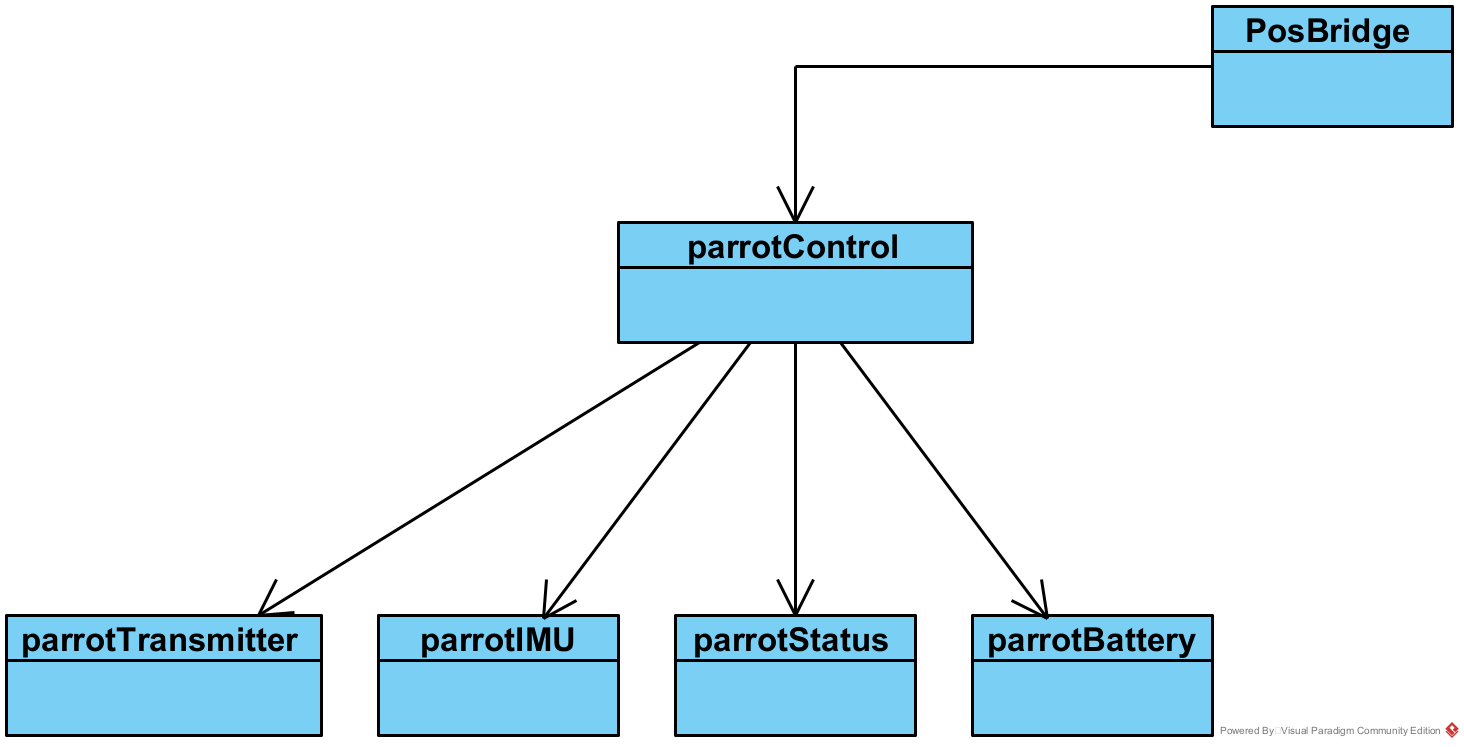
\includegraphics[width=12cm]{Pictures/Fassade.png}}
\caption{Fassade im Projekt}
\label{fig:Fas}
\end{center}

\vspace{0.25cm}
\end{figure}

\newSec[Akteure]{Akteure\footnotemark[3]}{4}
\begin{table}[!ht]
\begin{tabular}{ll}
Akteur			& Klassenbezeichnung \\ \hline
Fassade			& parrotControl\\
SubsystemKlasse 0	& parrotTransmitter\\
SubsystemKlasse 1	& parrotIMU\\
SubsystemKlasse 2	& parrotStatus\\
SubsystemKlasse 3	& parrotBattery\\
Subsystem B		& MainClass
\end{tabular}
\end{table}


\FloatBarrier
\newSec{Motivation}{4}
Für Dritte ist die Interaktionmit einer Klasse (Fassade) ist weniger kompliziert als die korrekte Initialisierung der von der Fassde gekapselten Klassen.
